% First draft - Phi 24. Nov 14
% version 0.2 - Tho 14. Dec 14
% version 0.3 - Phi 17. Dec 14
% Version 0.4 - Tho 24. Dec 14

\documentclass[final,reqno]{siamltex}

\usepackage{amsfonts,epsfig}
\usepackage{amsmath,amssymb} %$#
\usepackage{graphicx}

\usepackage[square, numbers, comma, sort&compress]{natbib}  % Use the "Natbib" style for the references in the Bibliography
%\usepackage{showlabels}
%\renewcommand{\showlabelfont}{\small\slshape\color{red}}

\usepackage{algorithm}
\usepackage{algpseudocode}
\usepackage{algcompatible}

\usepackage{xcolor}
\newcommand\command[1]{\textcolor{red}{\textbf{#1}}}

% %\usepackage[notcite]{showkeys}
% \usepackage{showlabels}
% \renewcommand{\showlabelfont}{\small\slshape\color{red}}

%\usepackage{lineno}
%\linenumbers

\usepackage{paralist}
\renewenvironment{itemize}[1]{\begin{compactitem}#1}{\end{compactitem}}
\renewenvironment{enumerate}[1]{\begin{compactenum}#1}{\end{compactenum}}
\renewenvironment{description}[0]{\begin{compactdesc}}{\end{compactdesc}}

\usepackage[pdfpagelabels]{hyperref} %$#

% Common extra environments
%\newtheorem{algorithm}[theorem]{Algorithm}
\newtheorem{remark}[theorem]{Remark}
\newtheorem{example}[theorem]{Example}
\newtheorem{ass}[theorem]{Assumption}
\newtheorem{hyp}[theorem]{Hypothesis}
\newtheorem{pro}[theorem]{Procedure}

%=============================================================================
% new def-s and commands
\newcommand{\reals}{\mathbb{R}}
\newcommand{\complex}{\mathbb{C}}

\def\leq{\leqslant}
\def\rar{\rightarrow}

\def\hro{\mathbb}
\def\R{\hro{R}}
\def\C{\hro{C}}
\def\N{\hro{N}}
\def\Z{\hro{Z}}
\def\bbI{\mathbb{I}}

\def\a{\alpha}
\def\ta{\widetilde{\alpha}}
\def\b{\beta}
\def\de{\delta}
\def\De{\Delta}
\def\tet{\theta}
\def\Tet{\Theta}
\def\dch{\dot{\chi}}
\def\ch{\chi}
\def\ka{\kappa}
\def\vp{\varphi}

\def\dtau{\Delta_{\tau}}
\def\idtau{\Delta_{-\tau}}

\def\ga{\gamma}
\def\Si{\Sigma}
\def\si{\sigma}
\def\om{\omega}
\def\lb{\lambda}
\def\fr{\frac}

\def\tp{\tilde{p}}
\def\tu{\tilde{u}}

\def\frE{\mathfrak{E}}
\def\frA{\mathfrak{A}}
\def\frB{\mathfrak{B}}
\def\frC{\mathfrak{C}}
\def\frD{\mathfrak{D}}
\def\frg{\mathfrak{g}}
\def\frf{\mathfrak{f}}
\def\frX{\mathfrak{X}}
\def\frZ{\mathcal{Z}}

\def\frM{\mathcal{M}}
\def\frP{\mathcal{P}}
\def\frG{\mathfrak{G}}
\def\tfrM{\tilde{\mathcal{M}}}
\def\tfrN{\tilde{\mathcal{N}}}
\def\tfrP{\tilde{\mathcal{P}}}
\def\tfrG{\tilde{\mathcal{G}}}

\def\hfrg{\hat{\mathfrak{g}}}
\def\tfrg{\tilde{\mathfrak{g}}}
\def\hmu{\hat{\mu}}

\def\bbM{\mathbb{M}}
\def\bbN{\mathbb{N}}

\def\hr{\hat{r}}
\def\hv{\hat{v}}
\def\hm{\hat{m}}
\def\hw{\hat{w}}

\def\tP{\tilde{P}}
\def\tQ{\tilde{Q}}
\def\tH{\tilde{H}}
\def\tK{\tilde{K}}

\def\tE{\widetilde{E}}
\def\hE{\hat{E}}
\def\tA{\widetilde{A}}
\def\hA{\hat{A}}
\def\bA{\breve{A}}
\def\tB{\widetilde{B}}
\def\hB{\hat{B}}

\def\hR{\hat{R}}
\def\hS{\hat{S}}
\def\hT{\hat{T}}

\def\tR{\tilde{R}}
\def\tS{\tilde{S}}
\def\tT{\tilde{T}}

\def\tU{\tilde{U}}
\def\tk{\tilde{k}}
\def\hk{\hat{k}}
\def\tX{\tilde{X}}
\def\hX{\hat{X}}
\def\bX{\breve{X}}

\def\tm{\tilde{m}}
\def\bM{\breve{M}}
\def\hM{\hat{M}}
\def\tM{\widetilde{M}}

\def\tmu{\tilde{\mu}}

\def\bE{\breve{E}}
\def\bA{\breve{A}}
\def\bB{\breve{B}}
%\def\uE{\u{E}}
%\def\uA{\u{A}}
%\def\uB{\u{B}}

\def\bbM{\mathbb{M}}
\def\btM{\widetilde{\mathbb{M}}}

\def\hW{\widehat{W}}
\def\tW{\tilde{W}}

\def\hN{\widehat{N}}
\def\tN{\widetilde{N}}

\def\cP{{\cal P}}
\def\cQ{{\cal Q}}
\def\cU{{\cal U}}

\def\cF{{\cal F}}
\def\cG{{\cal G}}
\def\hcF{\hat{\cF}}
\def\hcG{\hat{\cG}}

\def\hcP{\hat{\cP}}
\def\hcQ{\hat{\cQ}}



\def\hS{\widehat{S}}
\def\hZ{\widehat{Z}}
\def\hH{\hat{H}}
\def\hG{\hat{G}}

\def\tx{\tilde{x}}
\def\tf{\tilde{f}}
\def\hf{\hat{f}}
\def\brf{\breve{f}}
\def\brg{\breve{g}}
\def\baf{\bar{f}}
\def\tg{\tilde{g}}
\def\hg{\hat{g}}
\def\ha{\hat{a}}
\def\hd{\hat{d}}
\def\hu{\hat{u}}

\def\cg{\mathcal{g}}
\def\ti{\times}
\def\utau{\underline{\tau}}
\def\otau{\bar{\tau}}
\def\vtau{{\tau}}
%\def\vtau{\vec{\tau}}
\def\hga{\hat{\ga}}

\renewcommand{\th}[1]{t_{(#1)}}

\def\be{\begin{equation}}
\def\ee{\end{equation}}
\newcommand{\ben}{\begin{eqnarray}}
\newcommand{\een}{\end{eqnarray}}
\newcommand{\bens}{\begin{eqnarray*}}
\newcommand{\eens}{\end{eqnarray*}}
\def\bc{\begin{cases}}
\def\ec{\end{cases}}
\newcommand{\bsq}{\begin{subequations}}
\newcommand{\esq}{\end{subequations}}

\newcommand{\m}[1]{
\begin{bmatrix}
 #1
\end{bmatrix}
}

\renewcommand{\pm}[1]{
\begin{matrix}
 #1
\end{matrix}
}

\newcommand{\doublehat}[1]{%
    \widehat{\widehat{#1\,}}
    }

\newcommand {\mpar}[1]{\marginpar{\fussy\tiny #1}} % marginal notes
\newcommand{\tcal}[1]{%
    \widetilde{\cal{#1}}
    }

    \newcommand{\hcal}[1]{%
    \widehat{\cal{#1}}
    }

    \newcommand{\bcal}[1]{%
    \breve{\cal{#1}}
    }

\newcommand{\bsp}[1]{
\begin{split}
 #1
\end{split}
}
\def\ddt{\fr{\mathrm{d}}{\mathrm{d}t}}

\newcommand{\eproof}{\space
    {\ \vbox{\hrule\hbox{\vrule height1.3ex\hskip0.8ex\vrule}\hrule}}\\[0.2cm]}
    
\def\bce{\begin{compactenum}}
\def\ece{\end{compactenum}}

\newcommand {\corank}   {\mathop{\rm corank}\nolimits}
\newcommand {\range}  {\mathop{\rm range}\nolimits}
\newcommand {\corange}  {\mathop{\rm corange}\nolimits}
\newcommand {\kernel}   {\mathop{\rm kernel}\nolimits}
\newcommand {\cokernel} {\mathop{\rm cokernel}\nolimits}
%===============================================================================
%opening
\begin{document}

\title{A new solver for linear delay differential-algebraic equations\footnotemark[1]}

\author{Phi Ha\footnotemark[2] \and Vinh Tho Ma\footnotemark[2] and Volker Mehrmann\footnotemark[2]}

\renewcommand{\thefootnote}{\fnsymbol{footnote}}

\footnotetext[1]{This work was supported by DFG Collaborative Research Centre 910,
{\it Control of self-organizing nonlinear systems: Theoretical methods and concepts of application}}
\footnotetext[2]{ Institut f\"{u}r Mathematik, MA 4-5, TU Berlin, Stra\ss e des 17. Juni 136, D-10623 Berlin,
Germany; \{ha,mavinh,mehrmann\}@math.tu-berlin.de}

\maketitle

\newcommand{\thedate}{Version 0.4 \quad \today}

\begin{center}
\thedate
\end{center}

\vskip 0.2cm

\begin{abstract}
We discuss the new solver COLDDAE for the numerical solution of linear differential-algebraic equations (DDAEs) of retarded and neutral type. The implementation is mainly based on the results introduced in \cite{HaM14}. In the single delay case, the solver can handle noncausal systems, i.e., systems, where the solution does not only depend on the system's past and current states, but also future states.
\end{abstract}

\begin{keywords} Delay differential-algebraic equation, differential-algebraic equation, delay differential equations, method of steps, derivative array, classification of DDAEs.
\end{keywords}

\begin{AMS}
34A09, 34A12, 65L05, 65H10.
\end{AMS}

\pagestyle{myheadings}
\thispagestyle{plain}
\markboth{P. Ha and V. T. Ma and V. Mehrmann}{COLDDAE: a new solver for linear DDAEs}

\section{Introduction}
We discuss the new solver COLDDAE for the numerical solution of linear delay differential-algebraic equations (DDAEs) with variable coefficients of the following form
%
\bsq\label{eq1.1}
\be\label{eq1.1a}
 E(t)\dot{x}(t) = A(t)x(t) + \sum_{i=1}^k B_i(t) x(t-\tau_i(t)) + f(t), \quad t\in (t_0,t_f],
\ee
%
where $E,A, B_i \in C([t_0,t_f],\mathbb{R}^{m\times n})$,
$f\in C([t_0,t_f],\mathbb{R}^{m})$ and 
the delay functions $\tau_i \in C([t_0,t_f],\mathbb{R})$ satisfy $\tau_i(t) > 0$ for all 
$t\in [t_0,t_f]$. For later use in the index reduction procedure, we further assume that all these functions are sufficiently smooth. 

Setting $\utau := \min \{\tau_i(t)| \ t\in [t_0,t_f], \ i=1,\dots,k \}$ and $\otau := \max \{\tau_i(t)| \ t\in [t_0,t_f], \ i=1,\dots,k \}$, 
we assume that $\utau >0$, which is often referred in the literature \cite{BelC63,BakPT02} as the \emph{non vanishing delay} case. 
We further assume that $\otau < \infty$. Typically, to obtain a particular solution of the DDAE \eqref{eq1.1a}, one needs to provide a history function (or initial function)  $\phi \in C([t_0-\otau,t_0],\R^n)$ and prescribe
%
\be
 x(t) = \phi(t), \quad t\in [t_0,t_f).
\ee
%
\esq
%
We assume that \eqref{eq1.1} has a unique solution $x\in C((t_0,t_f],\mathbb{R}^n)$. For systems with constant delays 
the theoretical analysis for problems of the form \eqref{eq1.1} has been discussed in \cite{HaMS14,HaM14,Ha15}. These results, however, 
can be directly generalized to the case of time dependent delays under some minor assumptions on the delay functions  $\tau_i$. Therefore, the solver we discuss in this paper is intended for time dependent delays. 
The most important concepts presented in this work are the causality, the system type, the shift index and the strangeness index of the DDAE \eqref{eq1.1a}.

Under the assumption that the continuous, piecewise differentiable solution of the problem \eqref{eq1.1} exists and is unique, the implementation of the new 
solver is based on the regularization procedure introduced in \cite{HaM14}, which first determines the shift index and 
the strangeness index and then transforms the DDAE \eqref{eq1.1a} into a regular, strangeness-free formulation with the same solution set. 
Using this regularization procedure, we can also compute a consistent initial value, if $\phi(t_0)$ is not consistent, i.e., does not satisfy all (hidden) constraints, and apply any appropriate integration scheme on the 
resulting regular, strangeness-free DDAE. We implemented the Radau IIA method of order 5, which is a 3-stage collocation Runge-Kutta method, see \cite{HaiW91}.
%
%=======================================================================================================================================
\section{A brief survey of the basic results}
%=======================================================================================================================================
%
The numerical solution of DDAEs, until now, has only been considered for square systems, see e.g. 
\cite{AscP95,BakPT02,CamL09,GugH07,Liu99,ShaG06,TiaYK11,ZhuP97,ZhuP98}. 
For such systems, the solution is usually computed by the classical (Bellman) \emph{method of steps} \cite{Bel61,BelC63,BelC65}, which will be recalled below.\\
Since $\utau>0$, we have $[t_0,t_f] \subset \underset{j=1,\dots,\ell+1}{\cup} [t_0+(j-1)\utau,t_0+j\utau]$ 
with $\ell := \lfloor \fr{t_f-t_0}{\utau} \rfloor$.
For all $t \in [t_0,t_0+\utau]$, we have $t-\tau_i(t) \leq t_0 + \utau - \utau = t_0,$ and hence $x(t-\tau_i(t)) = \phi(t-\tau_i(t))$.
The DDAE \eqref{eq1.1a} restricted on the interval $[t_0,t_0+\utau]$ then becomes
%
\be\label{eq2}
 E(t)\dot{x}(t) = A(t)x(t) + \sum_{i=1}^k B_i(t) \phi(t-\tau_i(t)) + f(t).
\ee
% 
This system is a DAE in the variable $x_1 := x|_{[t_0,t_0+\utau]}$. The initial vector of the corresponding IVP for the DAE \eqref{eq2} is $x(t_0)=\phi(0)$, if consistent.
Supposing that this IVP has a unique solution $x_1$, we can proceed in the same way to compute the function $x_2 := x|_{[t_0+\utau,t_0+2\utau]}$, since 
$t-\tau_i(t) \leq t_0 + 2 \utau - \utau = t_0+\utau$, for all $t\in [t_0+\utau,t_0+2\utau]$. Therefore, the solution $x$ of \eqref{eq1.1} will be 
computed step by step on consecutive intervals $[t_0+(j-1)\utau,t_0+j\utau]$, $1\leq j\leq \ell$, by consecutively solving DAEs of the form
%
\be\label{eq3}
 E(t) \dot{x}_j(t) = A(t)x_j(t) + g_j(t) \quad \mbox{for all } t \in [t_0+(j-1)\utau,t_0+j\utau].
\ee
%
Clearly, we see that the method of steps successfully handles the problem \eqref{eq1.1} if and only if for every $j$, the corresponding IVP for the 
DAE \eqref{eq3} has a unique solution.
This requirement means that the solution $x$ at the current point $t'\in(t_0,t_f]$ depends only on the system \eqref{eq1.1a} 
at current and past time points $t \leq t'$, but not at future time points $t > t'$. We call this property \emph{causality}, and 
a DDAE that satisfies this property \emph{causal}. 
Restricted to the class of causal systems, different integration strategies based on the method of steps have been successfully implemented for 
linear DDAEs of the form \eqref{eq1.1a} and also for several classes of nonlinear DDAEs, see e.g. \cite{AscP95,BakPT02,GugH07,Hau97,ShaG06}.
In contrast to causal DDAEs, this approach is not feasible for noncausal systems,
consider for example the equation 
%
\be\label{eq2.1}
  0 \cdot \dot{x}(t) = 0 \cdot x(t) - x(t-\tau) + f(t), \quad \mbox{for all } t\in (0,\infty).
\ee
%
The method of steps applied to the DDAE \eqref{eq2.1} results in a sequence of underdetermined DAEs of the form
%
\[
 0 = g_i(t), \quad \mbox{for all } t \in [t_0+(j-1)\utau,t_0+j\utau]. 
\]
%
Nevertheless, \eqref{eq2.1} still has a unique solution. 
The reason for this failure is that the method of steps takes into account only the equation at the current time, which is not enough, 
due to the noncausality. Therefore, a regularization procedure for DDAEs, so that the method of steps can be used for the resulting systems, is 
necessary. Note that for noncausal DDAEs of the form \eqref{eq1.1a}, the solvability analysis has only been discussed for 
the single delay case, i.e., $k=1$. Even for multiple constant delays, i.e., $\tau_i(t) \equiv \tau_i$, the solvability analysis for noncausal DDAEs 
is not entirely understood, \cite{HaM14,Ha15}. 
The regularization procedure proposed in the package COLDDAE for causal and noncausal systems will be considered in the Subsections \ref{Sec2.1} and \ref{Sec2.2}, respectively.

\subsection{Regularization procedure for causal DDAEs with multiple delays}\label{Sec2.1}
Inherited from the theory of DAEs, we see that even for causal DDAEs, the numerical integration requires a reformulation of the original system in such a way that one can 
avoid the loss in order of convergence or the drift-off effect, see e.g. \cite{BreCP96,KunM06}. Here we use the regularization procedure 
associated with the \emph{strangeness index} concept, see \cite{KunM06}, which generalizes the well-known \emph{differentiation index} \cite{BreCP96} for general 
under- and over-determined DAEs. Briefly speaking, the strangeness index $\mu$ of the DAE 
%
\be\label{eq4}
 E(t)\dot{x}(t) = A(t)x(t) + f(t), 
\ee
%
is the minimum number of differentiations such that from the \emph{derivative array} (or \emph{differentiation-inflated} system)
%
\bens
 E(t)\dot{x}(t) - A(t)x(t)  &=& f(t), \\
 \ddt \left( E(t)\dot{x}(t) - A(t)x(t) \right) &=& f^{(1)}(t), \\
 & \dots & \\
 \left( \ddt \right)^{\mu} \left( E(t)\dot{x}(t) - A(t)x(t) \right) &=& f^{(\mu)}(t),
\eens
%
one can extract the so-called \emph{strangeness-free formulation}
%
\be\label{s-free form}
 \m{\hE_1(t) \\ 0 \\ 0} \dot{x}(t) = \m{\hA_1(t) \\ \hA_2(t) \\ 0} x(t) + \m{\hf_1(t) \\ \hf_2(t) \\ \hf_3(t)},
\ee
%
which has the same solution set as the DAE \eqref{eq4}, where the matrix-valued function $\m{\hE^T_1 & \hA^T_2}^T$ has pointwise full row rank.
We also call $\mu$ the strangeness index of the pair $(E,A)$. 
For the numerical determination of the strangeness index and the strangeness-free formulation \eqref{s-free form}, we refer the readers to 
\cite{KunMRW97,KunMS05}.

Now we apply this regularization procedure to the DDAE \eqref{eq1.1a}, which is assumed to be causal, and obtain the \emph{strangeness-free DDAE}
%
%\be\label{eq5}
 %\m{\hE_{1}(t) \\ 0 \\ 0} \dot{x}(t) \!=\! \m{\hA_{1}(t) \\ \hA_{2}(t) \\ 0} x(t) \!+\!
% \m{\hB_{0,1}(t) \\ \hB_{0,2}(t) \\ 0} x(t-\tau(t))
 %\!+\!  \sum_{j=1}^{\mu} \m{0 \\ \hB_{j,2}(t) \\ 0} x^{(i)}(t-\tau(t))
% \!+\! \m{\hf_{1}(t) \\ \hf_{2}(t) \\ \hf_{3}(t)}, \quad \pm{d \\ a \\ v}
%\ee
%
\begin{equation}\label{eq5}
\begin{aligned}
 \m{\hE_{1}(t) \\ 0 \\ 0} \dot{x}(t) =&
\m{\hA_{1}(t) \\ \hA_{2}(t) \\ 0} x(t) \!+\!
\sum_{i=1}^k \m{\hB_{i,0,1}(t) \\ \hB_{i,0,2}(t) \\ 0} x(t-\tau_i(t))\\&
 \!+\!  \sum_{i=1}^k\sum_{j=1}^{\mu} \m{0 \\ \hB_{i,j,2}(t) \\ 0} x^{(j)}(t-\tau_i(t))
 \!+\! \m{\hf_{1}(t) \\ \hf_{2}(t) \\ \hf_{3}(t)}, \quad \pm{d \\ a \\ v}
\end{aligned}
\end{equation}
The sizes of the block row equations are $d$, $a$, $v$. Due to the causality of the DDAE \eqref{eq1.1a}, it follows that $\m{\hE^T_1 & \hA^T_2}$ is pointwise 
nonsingular.
For the DAE \eqref{eq4}, the numerical solution $x(t)$ is obtained by integrating the strangeness-free formulation \eqref{s-free form}, which is more 
advantageous, see \cite{KunM96a,KunM96c,KunM06}.
For the DDAE \eqref{eq1.1a}, integrating the strangeness-free DDAE \eqref{eq5} is not always possible. The reason is that if 
at least one of the matrix functions $\hB_{i,j,2}$ is not identically zero, then the underlying DDE 
is of advanced type, which is not suitable for numerical integration, \cite{BelZ03}. In fact, until now there has been no solver for general advanced DDEs. 
For the numerical solution, solvers based on the method of steps are only suitable for retarded and neutral DDAEs, see \cite{AscP95,GugH07,Hau97,HaM14}.
In these cases, the strangeness-free DDAE \eqref{eq5} takes the form
%
\be\label{eq6}
 \m{\hE_{1}(t) \\ 0 \\ 0} \dot{x}(t) \!=\! \m{\hA_{1}(t) \\ \hA_{2}(t) \\ 0} x(t) \!+\!
 \sum_{i=1}^k\m{\hB_{i,1}(t) \\ \hB_{i,2}(t) \\ 0} x(t-\tau_i(t)) \!+\! \m{\hf_{1}(t) \\ \hf_{2}(t) \\ \hf_{3}(t)}, \quad \pm{d \\ a \\ v}.
\ee
%
The integration strategy we use for causal, retarded/neutral DDAEs of the form \eqref{eq1.1a} is: first, determine the strangeness-free formulation 
\eqref{eq6}, and second, apply numerical methods to \eqref{eq6} to compute $x(t)$.\\
Without loss of generality, we set $k=1$, $B(t):=B_1(t)$ and  $\tau(t):=\tau_1(t)$ for notational convenience.
For the determination of the strangeness-free DDAE \eqref{eq6}, we use the derivative array of the DDAE as follows.
%
\bens
 E(t)\dot{x}(t) - A(t)x(t)  &=& B(t)x(t-\vtau(t)) + f(t), \\
 \ddt \left( E(t)\dot{x}(t) - A(t)x(t) \right) &=& \ddt \left( B(t)x(t-\vtau(t)) + f(t) \right), \\
 & \dots & \\
 \left( \ddt \right)^{\mu} \left( E(t)\dot{x}(t) - A(t)x(t) \right) &=& \left( \ddt \right)^{\mu} \left( B(t)x(t-\vtau(t)) + f(t) \right),
\eens
%
which can be rewritten as
%
\be\label{eq7}
M(t) z(t) = P(t) z(t-\tau(t)) + g,
\ee
%
where 
%
\bens
&& M(t) := 
     \m{-A(t)    & E(t) & & & \\ 
    -\dot{A}(t)  & \dot{E}(t)-A(t) & E(t) & & \\ 
    -\ddot{A}(t) & \ddot{E}(t)-2\dot{A}(t) & 2\dot{E}(t)-A(t) & E(t) & \\ 
     & \vdots & & \ddots & \ddots & \\ 
-A^{({\mu})}(t)  & E^{({\mu})}(t)-{\mu}A^{({\mu}-1)}(t) & \dots  & \dots & {\mu}\dot{E}(t)-A(t) & E(t)}, \\
&& P(t)  := \m{B(t) &          &   &         &  & 0\\ 
 \dot{B}(t)    & B(t) (1-\dot{\tau}(t))        &   &         &  & 0\\ 
\ddot{B}(t)    & 2\dot{B}(t)(1-\dot{\tau}(t)) - B(t) \ddot{\tau}(t) & B(t)(1-\dot{\tau}(t))^{2} &         &  & 0\\ 
  \vdots       &  \vdots & \vdots &  & & \vdots \\ 
   *           & *       &   *    &  & & 0 
} \\
&& z(t) := \m{x(t) \\ \dot{x}(t) \\ \vdots \\ x^{(\mu+1)}(t)}, 
\quad g := \m{f(t) \\ \dot{f}(t) \\ \vdots \\ f^{(\mu+1)}(t)}.  
\eens
%
Note that the $j$-th block row of $P$ is obtained by computing the coefficients of
$\left({\ddt}\right)^{j-1}\left(B(t) x(t-\tau(t))\right)$, $j=1,\dots,\mu$. 
These coefficients can be computed by using Fa\`{a} di Bruno's formula \cite{Cra05}, which describes the $m$-th derivative of the 
composite function $g(f(x))$ in the variable $x$ as follows
%
\be\label{Faa di Bruno}
\bsp{
 & \left( \ddt \right)^m \left[ g(f(x)) \right] \\
 & = \sum \fr{m!}{b_1! \dots b_m!} g^{(k)}(f(x)) \left( \fr{f^{(1)}(x)}{1!}\right)^{b_1} \left( \fr{f^{(2)}(x)}{2!} \right)^{b_2} \dots 
 \left( \fr{f^{(k)}(x)}{k!} \right)^{b_k},
 }
\ee
%
where the sum is over all possible combinations of nonnegative integers $b_1,\dots,b_k$ such that $b_1+ 2b_2 + \dots+ mb_m = m$ and 
$k=b_1+b_2+\dots+b_m$. Note that, in our solver we assume that $\mu \leq 3$, therefore the entries of $P$ are hard coded.

In the following, for notational convenience, we will use Matlab notation, \cite{matlab}.
The set of algebraic constraints in the strangeness-free DDAE \eqref{eq6} is selected by finding the full row rank matrix $Z_2$ such that
%
\be\label{eq8}
 Z^T_2 M(:,(n+1):end) = 0.
\ee
%
Scaling the system \eqref{eq7} with $Z^T_2$ from the left, we obtain the equation
%
\be\label{eq9}
 Z^T_2 M(:,1:n) x(t) = Z^T_2 P z(t-\vtau(t)) + Z^T_2 g.
\ee
%
Furthermore, the DDAE \eqref{eq1.1a} is not of advanced type if and only if in \eqref{eq9} the derivatives of $x(t-\vtau(t))$ do not occur. This means 
that
%
\be\label{eq10}
 Z^T_2 P(:,(kn+1):end) = 0.
\ee
%
Consider the following spaces and matrices
%
\be\label{eq11}
\begin{array}{ccc} 
 T_2 & \mbox{ basis of } & \ker(Z^T_2 E), \\
 Z_1 & \mbox{ basis of } & \range(E T_2), \\
 Y_2 & \mbox{ basis of } & \range(Z^T_2 M(:,1:n)). \\
\end{array}
\ee
%
The set of differential equations in the strangeness-free DDAE \eqref{eq6} is then given by
%
\[
 Z_1^T E(t)\dot{x}(t) = Z_1^T A(t)x(t) + Z_1^T B(t) x(t-\vtau(t)) + Z_1^T f(t).
\]
%
In summary, we obtain the strangeness-free DDAE
%
\be\label{eq12}
 \bsp{
  Z_1^T E(t)\dot{x}(t) &=  Z_1^T A(t)x(t) +  Z_1^T B(t) x(t-\vtau(t)) +  Z_1^T f(t), \\
 Y^T_2 Z^T_2 M(:,1:n) x(t)  &= Y^T_2 Z^T_2 P(:,1:kn) x(t-\vtau(t)) + Y^T_2 Z^T_2 g,
 }
\ee
%
where $\m{Z_1^T E(t) \\ Y^T_2 Z^T_2 M(:,1:n)}$ is nonsingular. 

\subsection{Regularization procedure for noncausal DDAEs with single delay}\label{Sec2.2}
In order to handle noncausal DDAEs with single delay, in \cite{HaM14}, the authors proposed the concept of the \emph{shift index} as follows.
%
\begin{definition}\label{shift index}
Consider the problem \eqref{eq1.1}. For each $t\in \mathbb{I}$, consider the sequence $\{\th{j}| j\geq 0\}$, starting with $\th{0}=t$, 
determined via the equation 
%
\be\label{eq14}
 \th{j+1} - \tau(\th{j+1}) = \th{j}, \quad \mbox{for all } j\geq 0.
\ee
%
Then, the minimum number $\ka = \ka(t)$ such that the so-called \emph{shift-inflated} system
%
\be\label{eq13}
\bsp{
  E(\th{0}) \dot{x}(\th{0}) &= A(\th{0}) x(\th{0}) + B(\th{0}) x(\th{0} - \tau(\th{0})), \\  
  E(\th{1}) \dot{x}(\th{1}) &= A(\th{1}) x(\th{1}) + B(\th{1}) x(\th{1} - \tau(\th{1})), \\  
                            & \ \vdots  \\
  E(\th{\ka}) \dot{x}(\th{\ka}) &= A(\th{\ka}) x(\th{\ka}) + B(\th{\ka}) x(\th{\ka} - \tau(\th{\ka})),                            
}
\ee
%
uniquely determines $x(\th{0})$, is called the \emph{shift index} of the DDAE \eqref{eq1.1a} with respect to $t$.
\end{definition}

To guarantee the existence and uniqueness of the sequence $\{\th{j}| j\geq 0\}$ in Definition \ref{shift index}, we assume that for every $s \in (t_0,t_f)$ the equation
%
\be\label{shift equation}
 t -\tau(t) = s,
\ee
%
has a unique solution on the time interval $(s,t_f)$. 

\begin{remark}
If the DDAE \eqref{eq1.1a} is causal then the shift index $\ka$ is $0$ for all $t \in [t_0,t_f]$.
\end{remark}

Using \eqref{eq14}, we can rewrite the shift-inflated system \eqref{eq13} as
%
\be\label{eq15}
\bsp{
&\m{E(\th{0})    &                            &             &     \\
                 & E(\th{1})                  &             &     \\
                 &                            & \ddots      &      \\   
                 &                            &             & E(\th{\ka}) 
                 } \! \m{\dot{x}(\th{0}) \\ \dot{x}(\th{1}) \\ \vdots \\ \dot{x}(\th{\ka})} \\
& = 
\m{A(\th{0})     &                           &             &     \\
   B(\th{1})     & A(\th{1})                 &             &     \\
                 &            \ddots         & \ddots      &      \\   
                 &                          &B(\th{\ka}) & A(\th{\ka}) 
                 } \! \m{x(\th{0}) \\ x(\th{1}) \\ \vdots \\ x(\th{\ka})}
                 \!+\! \m{B(\th{0})x(\th{0}-\tau(\th{0})) \!+\! f(\th{0}) \\ f(\th{1}) \\ \vdots \\ f(\th{\ka})}.
}
\ee
%
As shown in \cite{HaM14}, assuming that the DDAE \eqref{eq1.1a} is not of advanced type and the strangeness index $\mu$ is well-defined for the DAE \eqref{eq15}, we can extract from the DAE \eqref{eq15} a strangeness-free DDAE 
%
\be\label{eq16}
 \m{\hE_{1}(\th{0}) \\ 0} \dot{x}(\th{0}) \!=\! \m{\hA_{1}(\th{0}) \\ \hA_{2}(\th{0})} x(\th{0}) \!+\!
 \m{\hB_{1}(\th{0}) \\ \hB_{2}(\th{0})} x(\th{0}-\tau(\th{0})) \!+\! \m{\hf_{1}(\th{0}) \\ \hf_{2}(\th{0})}, \ \pm{d \\ a}
\ee
%
where $\m{\hE_{1}(\th{0}) \\ \hA_{2}(\th{0})}$ is nonsingular.\\
Analogous to the case of causal DDAEs, we build the derivative arrays \eqref{eq7} for system \eqref{eq15}, and extract from it the 
strangeness-free DDAE \eqref{eq16}. To keep the brevity of the paper, we will not repeat the process.
It has been observed in \cite{HaM14} that the main differences between regularizing causal DDAEs and regularizing noncausal DDAEs are:
\begin{enumerate}
 \item[i)] The size of the derivative arrays \eqref{eq7} for noncausal DDAEs is bigger than for causal DDAEs.
 \item[ii)] For noncausal DDAEs the set of differential equations in the strangeness-free formulation \eqref{eq6} cannot be selected from the original DDAE \eqref{eq1.1a}, but must be 
 selected from the derivative array \eqref{eq7}.
\end{enumerate}

\section{Algorithms in COLDDAE}
First, we observe that the resulting system of the regularization procedure for DDAEs is the following regular, strangeness-free DDAE
%
\be\label{eq3.1}
 \m{\hE_1(t) \\ 0} \dot{x}(t) = \m{\hA_1(t) \\ \hA_2(t)} x(t) + \sum_{i=1}^k\m{\hB_{i,1}(t) \\ \hB_{i,2}(t)} x(t-\tau_i(t)) + \m{\hga_1(t) \\ \hga_2(t)}, 
\ee
%
where $k=1$ for noncausal DDAEs. We now apply numerical methods to \eqref{eq3.1} to determine $x(t)$.
Again, we set  $k=1$ also for the causal case without loss of generality and for notational convenience.
\\
Adopted from the solver RADAR5 \cite{GugH07}, we use the Radau scheme for the numerical integration, which is given by nodes
%
\be\label{eq3.2}
  0 < \de_1 < \dots < \de_s = 1, \quad s\in \hro{N}.
\ee
%
If we know all the discontinuity points of $\phi$, $\dot{\phi},\dots,\phi^{(s)}$ then we also know all the discontinuity points 
of $x$, $\dot{x},\dots,x^{(s)}$ on $[t_0,t_f]$, and hence we can include them into the mesh. 
However, for simplicity, the solver considers only the case that there is at 
most one discontinuity point at $t_0$. We denote a mesh by $\pi \ : \ t_0 < t_1 < \dots < t_N = t_f$.
The collocation points therefore are
%
\be\label{eq3.3}
  t_{ij} = t_i + h_i \de_j, \qquad j=1,\dots,s, 
\ee
%
where $h_i$ is the step size used at the $i$-th step.
For the numerical approximation of the solution, we seek for the piecewise polynomial $\mathrm{X}_{\pi}$ of degree $s$, i.e., 
$\mathrm{X}_{\pi,i}:=\mathrm{X}_{\pi}|_{[t_i,t_{i+1}]}$ are polynomials of degree $s$, which are determined by the following set of equations  
%
\be\label{eq3.4}
 \m{\hE_1(t_{ij}) \\ 0} \dot{\mathrm{X}}_{\pi}(t_{ij}) = \m{\hA_1(t_{ij}) \\ \hA_2(t_{ij})} \mathrm{X}_{\pi}(t_{ij}) + 
 \m{\hB_1(t_{ij}) \\ \hB_2(t_{ij})} \mathrm{X}_{\pi}(t_{ij}-\tau(t_{ij})) 
 + \m{\hga_1(t_{ij}) \\ \hga_2(t_{ij})}, 
%
\ee
%
for all $i=1,\dots,N$, $j=1,\dots,s$.\\
Due to the presence of $\m{\hB_1(t_{ij}) \\ \hB_2(t_{ij})} \mathrm{X}_{\pi}(t_{ij}-\tau(t_{ij}))$ in \eqref{eq3.4}, we still have to define the history function 
$\mathrm{X}_{\pi}(t_{ij}-\tau(t_{ij}))$ which is an approximation to $x(t_{ij}-\tau(t_{ij}))$. For this we choose
%
\[
\bsp{
&  \mathrm{X}_{\pi}(t_{ij}-\tau(t_{ij})) \\
 & =  
 \bc
  \phi(t_{ij}-\tau(t_{ij}))                & \mbox{if } t_{ij}-\tau(t_{ij}) < t_0, \\
  \mathrm{X}_{\pi,K}(t_{ij}-\tau(t_{ij}))  & \mbox{for $ 1 \leq K \leq N-1$ with } t_K < t_{ij}-\tau(t_{ij}) \leq t_{K+1}.
 \ec
} 
\]
%
The continuous output polynomial $\mathrm{X}_{\pi,K}$ at the $K$-th step is given by Lagrange interpolation of order $s$, i.e.,
%
\be\label{eq3.5}
 \mathrm{X}_{\pi,K}(t_K + \tet h_K) = \sum_{j=0}^s {\cal L}_j(\tet) \mathrm{X}_{\pi,K}(t_K + \de_j h_K),
\ee
%
where ${\cal L}_j(\tet)$ is the Lagrange polynomial of degree $s$ satisfying ${\cal L}_j(\de_K) = \de_{Kj}$ with $\de_{Kj}$ being the Kronecker delta symbol.

\begin{remark}
 As noticed in \cite{GugH01,GugH07}, one can optionally replace the continuous output polynomial $\mathrm{X}_{\pi,K}$ in \eqref{eq3.5} by another dense output polynomial given by
 %
 \[
  \mathrm{X}_{\pi,K}(t_K + \tet h_K) = \sum_{j=1}^s {\cal L}_j(\tet) \mathrm{X}_{\pi,K}(t_K + \de_j h_K).
 \]
 %
 The use of only $s$ interpolation nodes $\de_j$, $j=1,\dots,s$ instead of $s+1$ nodes $\de_j$, $j=0,\dots,s$ is beneficial in the presence of a jump in the solution at the
 point $t_K$, i.e., $\mathrm{X}_{\pi,K}(t_K) \not= \mathrm{X}_{\pi,K-1}(t_K)$.
\end{remark}

The existence and uniqueness, and the convergence results for the numerical approximation $\mathrm{X}_{\pi}$ are stated in the following theorem.

\begin{theorem}\label{Thm6.1}
Consider the problem \eqref{eq1.1} and assume that it is uniquely solvable and of either retarded or neutral type. 
For $N \in \hro{N}$ and $s \geq 1$, define the mesh $\pi$ and the collocation points $t_{ij}$, $j=1,\dots,s$ as in \eqref{eq3.3}. 
Then the following assertions hold.
\begin{compactenum}
 \item[i)] For sufficiently small mesh widths $h_0,\dots,h_{N-1}$ there exists one and only one continuous piecewise polynomial $\mathrm{X}_{\pi}$ that solves 
 the DAE sequence \eqref{eq3.4} and it is consistent at all the mesh point $t_i$.
 \item[ii)] The convergence order of the collocation method with schemes $\de_j$ as in \eqref{eq3.2} is $s$, i.e., 
 %
 \[
  \| \mathrm{X}_e(t) - \mathrm{X}_{\pi}(t) \|_{\infty} = \underset{t \in \bbI}{\sup} \| \mathrm{X}_e(t) - \mathrm{X}_{\pi}(t) \| = O(h^s),
 \]
%
 where $\mathrm{X}_e$ is the exact solution  $x \in C^{s+1}(\bbI,\C^n)$ to the problem \eqref{eq1.1}.
\end{compactenum}
\end{theorem}
\begin{proof}
For the proof see Theorem 4, \cite{Hau97} or Theorem 4.2, \cite{GugH07}.
\end{proof}
%

\section{Using COLDDAE}

The solver COLDDAE, implemented in Matlab, can handle both causal and noncausal DDAEs of retarded and neutral type, but as already stated above, we restrict the noncausal systems to have only one delay. If the system is of advanced type, an appropriate error message is thrown.
We have implemented step size control and so-called long steps, i.e.,  the step size may become bigger than the delay. 
Unless the user provides the exact derivative array, i.e. $M$, $P$ and $g$ from equation \eqref{eq7}, the strangeness index of the system \eqref{eq15} can be at most three due to hard coding in the computation of $P$.

In the following we will describe the parameters inside the solver.

\subsection{Input parameters}
\begin{itemize}
\item {\tt E}\quad The matrix function $E:[t_0,t_f]\rightarrow \mathbb{R}^{m,n}$.
\item {\tt A}\quad The matrix function $A:[t_0,t_f]\rightarrow \mathbb{R}^{m,n}$.
\item {\tt B}\quad The matrix function $B:[t_0,t_f]\rightarrow \mathbb{R}^{m,kn}$, where $k$ is the number of delays.
\item {\tt tau}\quad  The delay functions $t\mapsto [\tau_1(t),\ldots,\tau_k(t)]$.
\item {\tt phi}\quad The history function $\phi$, i.e.,  $x(t)=\phi(t)$ for $t < t_0$.
\item {\tt tspan}\quad The solution interval $[t_0,t_f]$, {\tt tspan(1)}$ = t_0$, {\tt tspan(2)}$ = t_f$ .
\item {\tt options}\quad A {\tt struct} containing the optional parameters.
\end{itemize}

\subsection{Optional input parameters}
Optional parameters can be passed by the input parameter {\tt options} by the command 
\begin{center}
{\tt options.}{\it field\_name} = {\it field\_value}.
\end{center}
The following fields are available in this solver:
\begin{itemize}
\item {\tt MaxIter}\quad        Upper bound for the total number of time steps (excluding 
	rejected time steps), default: {\tt 10000}.
\item {\tt MaxReject}\quad      Upper bound for the number of rejections per time step, default: {\tt 100}.
\item{\tt MaxCorrect}\quad  Upper bound for the number of correction steps when using
         long steps (step size bigger than the lag), default: {\tt10}.
\item {\tt InitStep}\quad        The initial step size of the Runge-Kutta method, default: $\frac{t_f-t_0}{100}$.
\item {\tt MinStep}\quad         A lower bound for the step size, default: $\tt 0$.
\item {\tt MaxStep}\quad      An upper bound for the step size, default: $\tt inf$.
\item {\tt AbsTol}\quad       Absolute tolerance, default:  {\tt 1e-5}.
\item {\tt RelTol}\quad       Relative tolerance, default:  {\tt 1e-5}.
\item {\tt StrIdx}\quad       Lower bound for the strangeness index,  default: {\tt 0}.
\item {\tt MaxStrIdx}\quad    Upper bound for the strangeness index,  default: {\tt 3}.
\item {\tt Shift}\quad       Lower bound for the strangeness index,  default: {\tt 0}.
\item {\tt MaxShift}\quad    Upper bound for the strangeness index,  default: {\tt 3}.
\item {\tt InitVal  }\quad    Initial value, not necessarily consistent,  default: $\phi(t_0)$.
\item {\tt IsConst}\quad   A boolean, {\tt true} if $E,A,B,\tau$ are constant, the regularized system is then computed only once, default: {\tt false}.
\item {\tt DArray}\quad    Struct with three fields containing $M$, $P$ (or $[P_1,\ldots,P_k]$ for $k>1$) and $g$ from equation \eqref{eq7}.  default: not set.
\end{itemize}

\subsection{Output parameters}
\begin{itemize}
\item {\tt t}\quad A discretization of {\tt tspan} with variable step size.
\item {\tt x}\quad The numerical solution at {\tt t}.
\item {\tt info}\quad A struct with information, e.g. the strangeness index, shift index, etc.
\end{itemize}

\section{Numerical experiments}
We use COLDDAE with its default values to solve four different non-advanced DDAEs. 
Example \ref{Exa1}, \ref{Exa2} are taken from the DDE test set \cite{Pau94}.
%
\begin{example}\label{Exa1} We consider the following DDE with constant delay.
%
\bsq\label{eq20}
\begin{equation}\label{eq20a}
\bsp{
\dot{x}_1(t) & = x_3(t),\\
\dot{x}_2(t) & = x_4(t),\\
\dot{x}_3(t) & = -2mx_2(t)+(1+m^2)(-1)^mx_1(t-\pi),\\
\dot{x}_4(t) & = -2mx_1(t)+(1+m^2)(-1)^mx_2(t-\pi),
}
\end{equation}
for $t>0$ and $x(t)=\phi(t)$ for $t\leq 0$ with 
\begin{equation}\label{eq20b}
\bsp{
{\phi}_1(t) & = \sin(t)\cos(mt),\\
{\phi}_2(t) & = \cos(t)\sin(mt),\\
{\phi}_3(t) & = \cos(t)\cos(mt)-m\sin(t)\sin(mt),\\
{\phi}_4(t) & =m\cos(t)\cos(mt)-\sin(t)\sin(mt).
}
\end{equation}
\esq
%
{\bf Analytical solution:} \quad $x(t)=\phi(t)$ for $t>0$.\\
The relative error of the numerical solution of \eqref{eq20} with $m=2$ is presented in Figure \ref{fig_Paul}.
\end{example}
%
\begin{example}\label{Exa2} We consider the following DDAE
%
\begin{equation}\label{eq21}
\begin{aligned}
\m{
1&-1\\
0&0 
}
\dot{x}(t) &=
\m{
1& 0\\
0&1 
}
x(t) + 
\m{
0& 0\\
-1&0
}
x(t-1), && \mbox{for all } t>0,\\
\phi(t) &=
\m{
1\\
0 
},
&& \mbox{for all } t \leq 0.
\end{aligned}
\end{equation}
%
Note that the DDAE \eqref{eq21} is reformulated from the neutral DDE $\dot{x}(t)=x(t)+\dot{x}(t-1)$ by introducing a new variable to present $x(t-1)$.\\
{\bf Analytical solution:}\quad The problem \eqref{eq21} possesses the unique solution 
$x(t)= \m{x_1(t) \\ x_2(t)}$ given by
\begin{align*}
x_1(t)=
\bc
\begin{array}{ll}
e^t & \mbox{ for } 0<t\leq1, \\
(t-1)e^{t-1}+e^t & \mbox{ for } 1<t\leq2, \\
\tfrac12(t^2-2t)e^{t-2}+(t-1)e^{t-1}+e^t & \mbox{ for } 2<t\leq3,\\
\tfrac16(t^3-3t^2-3t+9)e^{t-3}+\tfrac12 (t^2-2t)e^{t-2}+(t-1)e^{t-1}+e^t & \mbox{ for } 3<t\leq4,
\end{array}
\ec
\end{align*}
and
$x_2(t)=x_1(t-1)$. The relative error of the numerical solution of \eqref{eq20} is also presented in Figure \ref{fig_Paul}.

\begin{figure}[h]
 \centering
 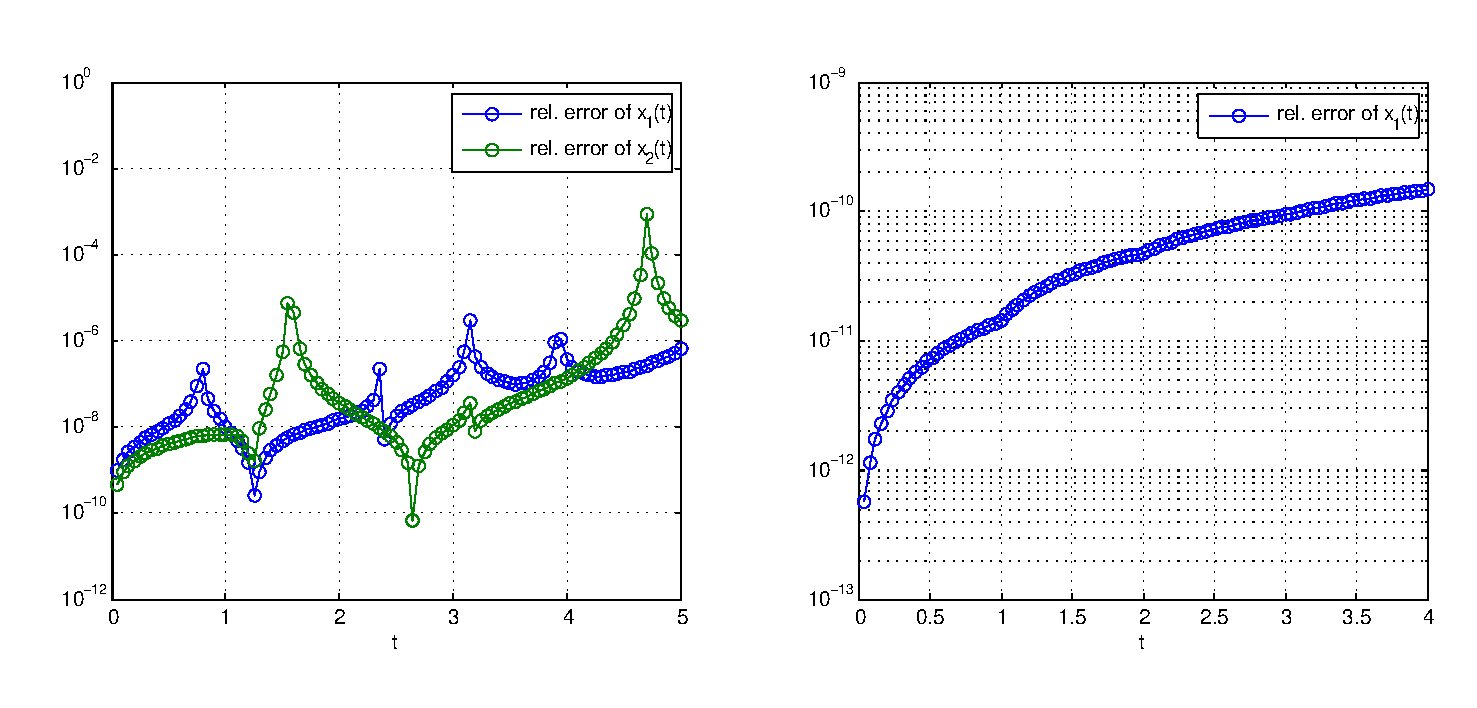
\includegraphics[width=\textwidth]{plot_149_214.pdf}
 % Paul_149.pdf: 0x0 pixel, 300dpi, 0.00x0.00 cm, bb= 
 \caption{Relative error of the solution of \eqref{eq20} (left) and \eqref{eq21} (right).}
 \label{fig_Paul}
\end{figure}
\end{example}

\begin{example} 
We consider the following DDAE with constant coefficients and multiple time-varying delays. This DDAE is causal and it has 
strangeness index two.
%
\begin{equation}\label{eq22}
\begin{aligned}
\m{
0&1&0\\
0&0&1 \\
0&0&0 
}
\m{\dot{x}_1(t) \\ \dot{x}_2(t) \\ \dot{x}_3(t)} &=
\m{x_1(t) \\ x_2(t) \\ x_3(t)} + 
\m{
x_2(t-1)+x_3(\tfrac t2-1)\\
0\\
0
}
+f(t), && \mbox{for all } t>0,\\
\phi(t) &=
\m{
e^t\\
1\\
\sin(t)
},
&& \mbox{for all } t \leq 0.
\end{aligned}
\end{equation}
The function $f(t)$ is chosen such that the analytical solution is $x(t)=\phi(t)$. The relative error of the numerical solution of \eqref{eq22} is presented in Figure \ref{fig_222}.
\end{example}

\begin{example} We consider the following linear DDAE with constant coefficients and time-varying delay. This DDAE 
is noncausal and it has strangeness index one and shift index one.
%
\begin{equation}\label{eq23}
\begin{aligned}
\m{
1&0\\
0&0 \\
}
\m{\dot{x}_1(t) \\ \dot{x}_2(t)} &=
\m{
0&0\\
1&0 \\
}
\m{x_1(t) \\ x_2(t)} + 
\m{
0&1\\
0&1
}
\m{x_1\bigl(t-1+\frac{\sin(t)}2\bigr) \\ x_2\bigl(t-1+\frac{\sin(t)}2\bigr)}
+f(t), && \mbox{for all } t>0,\\
\phi(t) &=
\m{
\sin(t)\\
\cos(t)
},
&& \mbox{for all } t \leq 0.
\end{aligned}
\end{equation}
The function $f(t)$ is chosen such that the IVP \eqref{eq23} has the unique solution $x(t)=\phi(t)$.
The relative error of the numerical solution of the IVP \eqref{eq23} is also presented in Figure \ref{fig_222}.
%
\begin{figure}[h!]
 \centering
 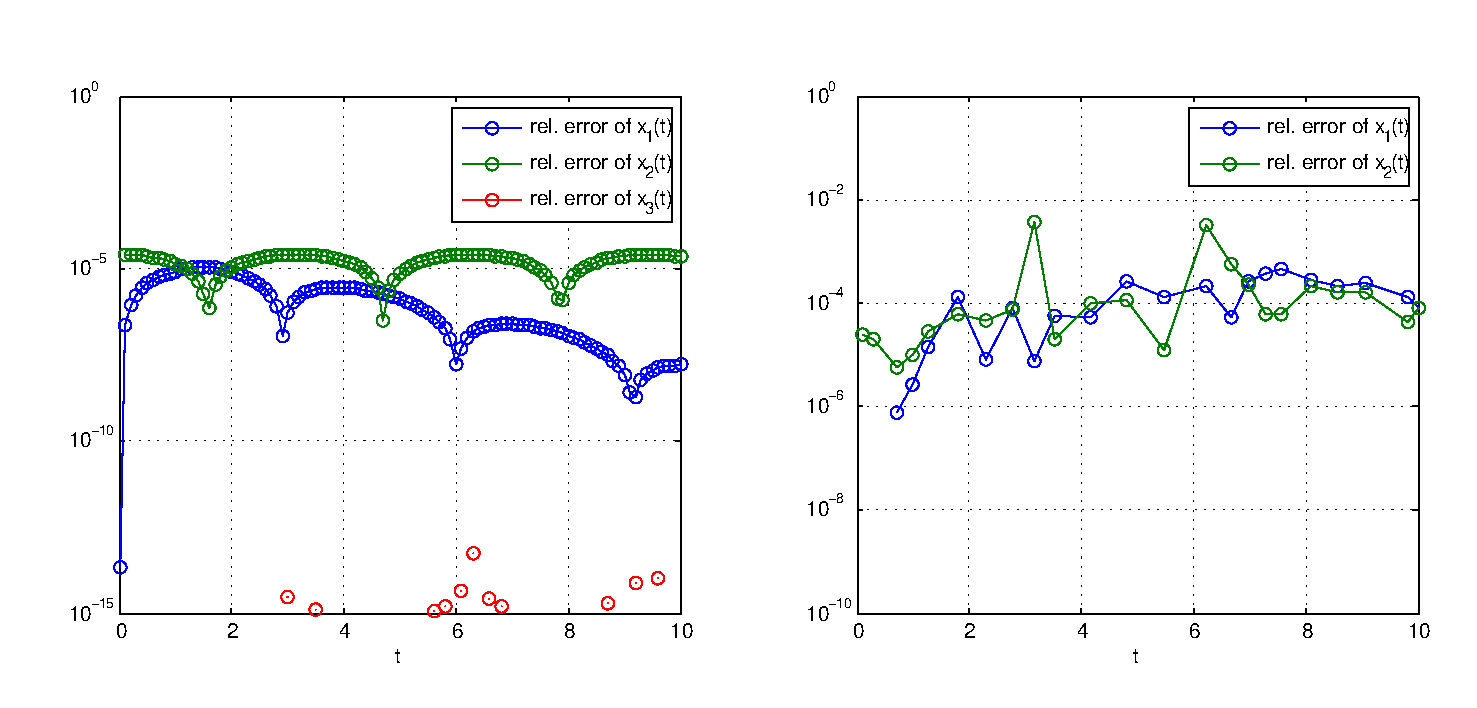
\includegraphics[width=\textwidth]{plot_222_varshifted.pdf}
 % Paul_149.pdf: 0x0 pixel, 300dpi, 0.00x0.00 cm, bb= 
 \caption{Relative error of the solution of \eqref{eq22} (left) and \eqref{eq23} (right).}
 \label{fig_222}
\end{figure}
\end{example}
%
% \section{Future work}
% Possible improvements include
% \begin{enumerate}
% \item regularization of non-causal DDAEs with multiple delays,
% \item step size control and long steps for multiple delays,
% \item using exact derivatives for the regularization (provided by user).
% \end{enumerate}

\section*{Acknowledgment} The first two authors would like to thank Benjamin Unger for useful 
suggestions and comments.

%-------------------------------------------------------------------------------
\bibliographystyle{plain}
%\bibliography{HaMM14}
\bibliography{Phi_Dec_15_14}
%-------------------------------------------------------------------------------
%%%%%%%%%%%%%%%%%%%%%%%%%%%%%%%%%%%%%%%%%%%%%%%%%%%%%%%
\end{document}
%%%%%%%%%%%%%%%%%%%%%%%%%%%%%%%%%%%%%%%%%%%%%%%%%%%%%%%
